\section{Trade-Offs for Multiple Stakeholders in LTE Video Transmission}\label{sec:application:lte_video}

\newcommand{\bandwidth}{\ensuremath{b_W}\xspace}
\newcommand{\bitrate}{\ensuremath{b_R}\xspace}
\newcommand{\timeplayedback}{\ensuremath{t_p}}

\newcommand{\streamingstart}{\ensuremath{\sigma}\xspace}
\newcommand{\bufferlower}{\ensuremath{\theta}\xspace}
\newcommand{\buffersize}{\ensuremath{\Theta}\xspace}

\newcommand{\ton}{\(T_{\texttt{ON}}\)\xspace}
\newcommand{\tdrxinactivity}{\(T_{\texttt{I}}\)\xspace}

\newcommand{\shortdrx}{\texttt{Short} \texttt{DRX}\xspace}
\newcommand{\tshortdrx}{\(T_{\texttt{S}}\)\xspace}
\newcommand{\longdrx}{\texttt{Long} \texttt{DRX}\xspace}
\newcommand{\tlongdrx}{\(T_{\texttt{L}}\)\xspace}
\newcommand{\rrcconnected}{\texttt{RRC\_Connected}\xspace}
\newcommand{\tidle}{\(T_{\texttt{Idle}}\)\xspace}
\newcommand{\tonidle}{\(T^{\texttt{Idle}}_{\texttt{ON}}\)\xspace}
\newcommand{\rrcidle}{\texttt{RRC\_Idle}\xspace}
\newcommand{\tdrxidle}{\(T^{\texttt{Idle}}_{\texttt{\gls{DRX}}}\)\xspace}
\newcommand{\promotiondelay}{\(D_P\)\xspace}

\newcommand{\bandwidthdown}{b_d\xspace}
\newcommand{\timedownloaded}{\ensuremath{t_d}}

\newcommand{\power}{P\xspace}
\newcommand{\energyconsumption}{\ensuremath{E}\xspace}
\newcommand{\connectioncount}{\ensuremath{C}\xspace}

\newcommand{\factordown}{\ensuremath{\alpha}\xspace}
\newcommand{\powerbaseline}{\ensuremath{\beta}\xspace}

\newcommand{\userabortrv}{\ensuremath{A}\xspace}
\newcommand{\userabortpdf}{\ensuremath{a}\xspace}
\newcommand{\meanwastedtraffic}{\ensuremath{W}\xspace}

\newcommand{\timeunwatched}{\ensuremath{t_u}}
\newcommand{\videolength}{l\xspace}

The delivery of video content in a mobile scenario is one of the major use cases for the \gls{LTE} mobile communication technology.
While the use of \gls{LTE} affords sufficient bandwidth to enable video playback in high definition, it also introduces new challenges for all stakeholders.
Similarly to the applications discussed in \refchap{chap:network}, signalling traffic induced by the video transmission may pose a challenge for mobile network operators, and power drain remains an open issue for hardware vendors.
Additionally, mobile playback can cause new problems for video providers.
Users watching video on the go may be prone to higher rates of interrupted video playback, either due to insufficient network coverage or social interactions.
If the video transmission mechanism has transmitted too much video content in advance, this transmitted data is ``wasted'', from the perspective of the video provider, as this consumes both network and computation resources but results in no benefit for the customer.

In \refsec{sec:application:lte_video:system_model} we present models for both video playback and the mobile network.
Then, in \refsec{sec:application:lte_video:numerical_evaluation} we perform a simulative study using the proposed model in order to evaluate the performance of the studied video transmission mechanisms.

\subsection{System Model}\label{sec:application:cloud_file_synchronisation:system_model}
This section first provides a general overview over the Dropbox service architecture and introduces the considered usecase.
Then, we propose the cloud storage model and metrics used in this analysis.
Finally, we discuss a set of scheduling mechanisms used to start the file synchronisation process. 

The authors of~\cite{Drago2012} provide a first study of the \dropbox architecture, which is schematically depicted in \reffig{fig:application:cloud_file_synchronisation:system_model:dropbox_architecture} and used as a basis for the model under study in the remainder of this section.

\begin{figure}
  \centering
  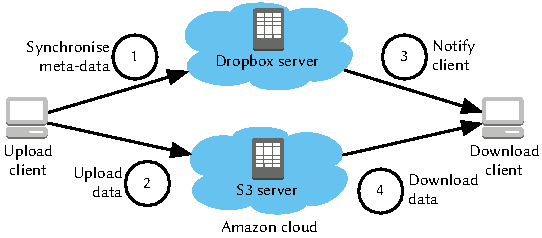
\includegraphics[width=\columnwidth]{application/cloud_file_synchronization/system_model/figures/dropbox_architecture}
  \caption{\dropbox file storage and retrieval process}
  \label{fig:application:cloud_file_synchronisation:system_model:dropbox_architecture}
\end{figure}

The \dropbox infrastructure consists of two main components:
\begin{enumerate*}
\item a storage cloud based on Amazon's Elastic Compute Cloud and Simple Storage Service, and 
\item (2) control servers directly maintained by \dropbox Inc. 
\end{enumerate*}

The control servers store meta information about the current state of the files in the \dropbox folders and trigger synchronization processes on the clients.

A file synchronization can basically be described in five steps.
As soon as the new file is added to the \dropbox folder of the uploading client, a preprocessing step is triggered and the meta information for the file are generated, respectively updated.
This information is then synchronized with the control servers~(1) and the file itself is uploaded to the storage cloud~(2).
After the file has completely been transferred to the storage cloud, all connected clients are notified about the update~(3) and start downloading the new file~(4).

\subsubsection*{Use Case: Photo Uploading}\label{sec:application:cloud_file_synchronisation:use_case}
In this section we consider the synchronization of images from a digital camera to a mobile \gls{UE} via a cloud storage provider.
Real world examples of this scenario are, e.g., taking photos of a live event and transferring them to a picture agency, or shooting private holiday images. 

The user took a finite set of pictures with a wearable device like Google Glass or a smart camera, e.g. a Nikon Coolpix S800c or SAMSUNG CL80.
The camera is then connected via a \gls{PAN} with a mobile \gls{UE}, for example a Laptop with a data card or a smartphone, to store the images on the mobile device.
The \gls{UE} uses broadband wireless Internet access technology and runs software provided by the cloud storage provider in order to synchronise the images with the cloud storage.
Finally, the scenario includes a remote client, which is connected using a wire line connection and downloads the images from the cloud.

For the evaluation presented in this paper, we consider a specific realization of the use case described above.
For the role of the cloud storage provider we consider \dropbox, Bluetooth is used as the technology for establishing the \gls{PAN}, and \gls{LTE} is used as the wireless broadband access technology.

In the considered scenario the interests of two stakeholders are impacted.
The first stakeholder, the end user, has two contradicting requirements on the system.
On the one hand side, the images should be synchronised as fast as possible. 
This requires a fast and permanent Internet connection of the \gls{UE}, which in turn is very power intensive.
On the other side, the power drain of the mobile device should be minimized to enable a long battery life time.
The second stakeholder, the mobile network provider, wants to minimize the signallisation overhead in the network~\cite{NSN2011, Huawei2011} caused by short time connections.
Here, an optimisation problem arises to find a practical solution for all three requirements. 
In order to analyse this problem, we use a simulation model of the file synchronization process, which is described in the following.

\subsubsection*{Cloud Storage Model and Performance Metrics}\label{sec:application:cloud_file_synchronisation:system_model:model_metrics}
The proposed simulation model is schematically depicted in \reffig{fig:application:cloud_file_synchronisation:system_model:model_metrics:model} and based on the findings of~\cite{Drago2012} described in~\refsec{sec:application:background}.

\begin{figure}
\centering
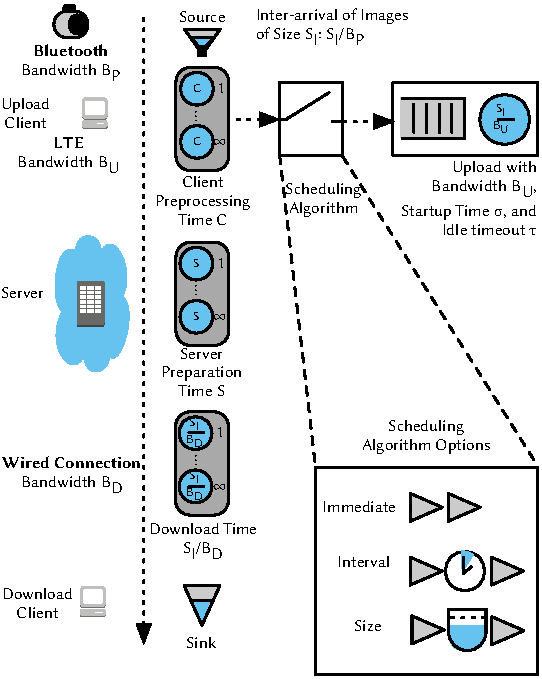
\includegraphics[width=\columnwidth]{application/cloud_file_synchronization/system_model/figures/model}
\caption{Synchronization Process Model}
\label{fig:application:cloud_file_synchronisation:system_model:model_metrics:model}
\end{figure}

We assume that the user has taken pictures of varying file size distributed with \imageFileSize.
These pictures are transfered from the camera to the mobile device using the \gls{PAN} with a constant bandwidth~\panTransferRate.
Due to the limited bandwidth \panTransferRate of the \gls{PAN} device, the inter-arrival times of images at the \dropbox shared folder of the mobile device can be calcluated by \(\interarrivaltime = \frac{\imageFileSize}{\panTransferRate}\).

As soon as the image is fully copied to the \dropbox folder, the generation of the meta data introduces a preprocessing delay, which we refer to as client preparation time~\clientpreparationtime.
To evaluate different strategies optimising the overall waiting time, power drain, and signallisation traffic we include a scheduling component.
This component implements different algorithms, described in \refsec{sec:application:cloud_file_synchronisation:system_model:algorithms}, which decide when the images currently held available in the scheduling component should be sent to the component responsible for transmission.

Next, we consider the \gls{LTE} \gls{UE} used for image upload.
Due to the specification of the \gls{LTE} standard \cite{3GPP_RRC_Spec}, the upload component can, at any point in time, either be connected to the mobile network or disconnected.
If the \gls{UE} is currently disconnected, and a new image for upload arrives, the connection process is triggered and completed after a startup delay \(\startupDelay = \SI{0.26}{\second}\).
Once the \gls{UE} is connected, arriving images are transmitted in order.
The transmission, i.e. service time, of an image depends on the size of the image currently being uploaded as well as the upload bandwidth \uploadbandwidth.
As only one image is transferred at once, waiting images are stored in a queue of infinite size.
If the \gls{UE} is idle for more than \(\idleThreshold = \SI{11.576}{\second}\), the device disconnects from the network.

After the image has been successfully uploaded to the storage servers, a server side preprocessing phase starts, before the file transfer to the downloading client starts.
This server side preprocessing again introduces an additional delay, the server preparation time~\serverpreparationtime, in the synchronization process.
Finally, the image is downloaded by the wire line client.
Again, the duration is calculated based on the size of the image and the available download bandwidth~\downloadbandwidth.

Next, we discuss the metrics used to evaluate the performance of the scheduling algorithms under consideration.
First, we consider the mean synchronization time \sojournTime, i.e., the time between the generation of images and the completion of the download.
This metric accounts for the desire of end users to synchronize images in a short amount of time.
Secondly, we study the relative amount of time the \gls{UE} is disconnected \relativeDisconnectedTime.
As the \gls{UE} consumes more power in the connected state, the user is generally interested in scheduling mechanisms which ensure that the device is only connected if required \cite{Ickin2012}.
This measure also enables a more general evaluation then the actually consumed power, as the concrete power drain differs significantly for each device.
Finally, we evaluate the number of transitions~\connectionCount between the connected and disconnected states.
As discussed in \refsec{chap:network}, frequent state transitions put a strain on the network due to increased signallling.
Thus, scheduling algorithms with a small number of transitions would be favored by network operators.

\subsubsection*{Scheduling Algorithms}\label{sec:application:cloud_file_synchronisation:system_model:algorithms}
We use different scheduling strategies in our model to control the uploading of the files from the mobile client.
These mechanisms in turn affect the synchronization time, the power drain, and the generated signalling traffic.

The most basic strategy of handing the upload is to immediately send new files, as soon as the meta data is generated.
We refer to this as \algoimmediate strategy and will use this as base line for all comparisons in the evaluations.
The other two strategies considered are based on a temporal, respectively a size threshold. 
Using the \algointerval scheduling, the client checks periodically if new files have been marked for synchronization.
If new files are present, they are synchronized to \dropbox.
Files which could not be sent within the current interval will automatically be added to the file batch for the next interval. 
The last scheduling mechanisms uses a threshold based on the overall \algosize of the images not yet synchronized.
If the threshold is crossed, an upload is triggered.

\subsection{Numerical Evaluation}\label{sec:application:lte_video:numerical_evaluation}

In this section we study the metrics introduced in \refsec{sec:application:lte_video:system_model:model_assumptions:metrics} on the different transmission mechanisms.

First, we study the impact of the considered transmission mechanisms on the energy consumption and the wasted traffic. 
Then, we consider the impact of the connection count for the \streaming mechanisms and varying values of the parameters \emph{stop threshold} \bufferlower and \emph{threshold size} \buffersize in more detail.

We consider a video of \(\videolength=\SI{1600}{\second}\) length which is viewed on a \gls{UE} with \gls{LTE} access.
The median of available downlink throughput in current \gls{LTE} networks is \(\bandwidth = \SI{12.74}{\mega\bit\per\second}\) \cite{Huang2012}.
A wide set of video bitrates between \SIlist{1;50}{\mega\bit\per\second} is in use~\cite{YouTube2013}.
In order to prevent stalling, we consider bitrates between \SIrange{1}{10}{\mega\bit\per\second}, staying below the available network bandwidth.
For the \streaming mechanism, a stop threshold of \(\bufferlower = \SI{4}{\second}\) and a threshold size of \(\buffersize = \SI{32}{\second}\) were selected.
Furthermore, we specify a prebuffering duration of \(\streamingstart = \SI{5}{\second}\).

We conduct our study using deterministic discrete event simulation which uses no random variables.
The wasted traffic is obtained analytically using the abort behaviour model.
Thus, all results are exact under the previously stated assumptions.

\subsubsection*{Energy Consumption}\label{sec:application:lte_video:numerical_evaluation:energy_consumption}
First, we study the influence of both video bitrate as well as the selected download mechanism on energy consumption in \reffig{fig:application:lte_video:numerical_evaluation:energy_consumption:bitrate2energy}.
\begin{figure}
  \centering
  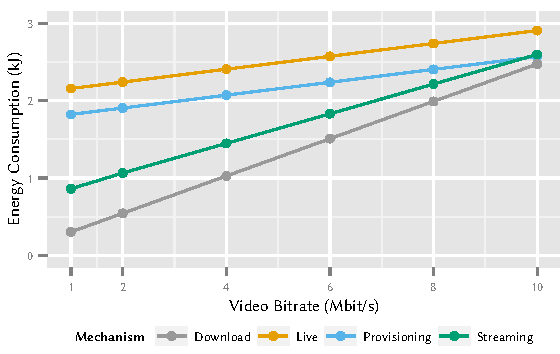
\includegraphics{application/lte_video/numerical_evaluation/figures/bitrate2energy}
  \caption{Influence of bitrate and download mechanism on energy consumption.}
  \label{fig:application:lte_video:numerical_evaluation:energy_consumption:bitrate2energy}
\end{figure}

We consider the \download mechanism and observe that it consumes the least amount of energy.
Here the video is downloaded with full bandwidth, as seen in \reffig{fig:application:lte_video:system_model:video_model}, resulting in a very short energy intensive download phase and a longer energy unintensive playback phase.
For the \live mechanism we observe the opposite, i.e. the highest energy consumption for all bandwidths.
If this mechanism is used, the used bandwidth equals the video bitrate.
Thus, the download requires the same amount of time as the playback, resulting in the highest possible energy consumption.
The \serviceprovisioning method uses a higher bandwidth, thus reducing the overall download time.
This reduced download time decreases the energy consumption when compared to the \live mechanism, even though the bandwidth used for downloading is increased to \SI{120}{\percent}.
For the \streaming mechanism we observe an energy consumption slightly higher than the \download mechanism.
As the bitrate of the video increases, the energy consumption increases as well.
This is due to the fact that a higher video bitrates require larger downloads.
For video bitrates approaching the available bandwidth the \streaming mechanism degenerates to the \live mechanism, as no prebuffering is possible.
We conclude that the \download and \streaming mechanisms outperform \live and \serviceprovisioning with regard to energy consumption.

\subsubsection*{Wasted Traffic}\label{sec:application:lte_video:numerical_evaluation:wasted_traffic}
Next, we consider the wasted traffic as a metric of the transmission mechanism quality.
If a user completely watches a video, no traffic is wasted, as all data downloaded is used during playback.
Thus, we consider only the cases where a user stops the playback before the video is finished.

\begin{figure}
  \centering
  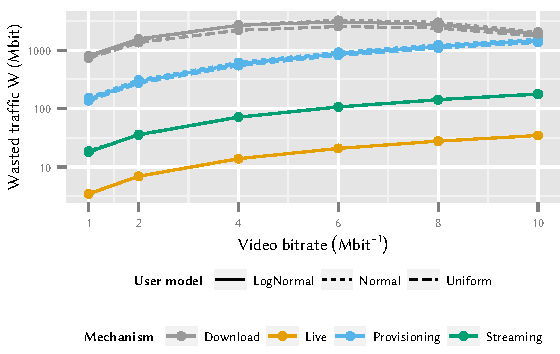
\includegraphics{application/lte_video/numerical_evaluation/figures/bitrate2lostData}
  \caption{Influence of bitrate, download mechanism and user model on wasted traffic. Download, Live, and Provisioning mechanisms result in equal connection counts.}
  \label{fig:application:lte_video:numerical_evaluation:energy_consumption:bitrate2lostData}
\end{figure}

In \reffig{fig:application:lte_video:numerical_evaluation:energy_consumption:bitrate2lostData} we study the wasted traffic for different video bitrates.
We consider the different transmission mechanisms introduced in \refsec{fig:application:lte_video:system_model:video_model} as well as the previously introduced user models.
We observe that the choice of user model has no significant impact on the wasted traffic.
For the \download mechanism, the amount of wasted traffic increases up to a video bitrate of \SI{6}{\mega\bit\per\second}, then the wasted traffic decreases as only video data which has been prebuffered can be lost if the user aborts the video.
As we assume an available bandwidth of \SI{12.74}{\mega\bit\per\second}, the bandwidth available for prebuffering decreases as the bitrate increases, resulting in lower amounts of wasted traffic for high video bitrates.
For the \live mechanism, we see that the wasted traffic for all user models is very low, but wasted traffic exists.
This is due to the traffic already sent by the server while the \gls{UE} is still waiting for promotion from \rrcidle to \rrcconnected, i.e. a short prebuffering phase exists.
As the bandwidth increases with the video bitrate, the wasted traffic increases as well.
Next, we consider the \serviceprovisioning approach and see an increase of wasted traffic as the video bitrate increases, due to the fact that the bandwidth used for continuous download is a factor of the video bitrate.
A higher video bitrate results in the download of the video being completed earlier, which leads to more wasted traffic.
Similar results can be seen for the \streaming mechanism, which results in more wasted traffic than the \live mechanism, but significantly less traffic than the \serviceprovisioning mechanism.
This is due to the fact that if the user aborts, at least the amount of video given by the \emph{stop threshold} \bufferlower and at most the complete buffer, given by the \emph{stop threshold} and the \emph{threshold size} are lost.
We have observed that the choice of user model results in no qualitative changes in wasted traffic.
As described in the last paragraph, the \download and \streaming mechanisms provide best results with regard to energy consumption.
However with regard to wasted traffic, the \live and \streaming mechanisms are most suited.
Thus, the \streaming mechanism seems to be a good compromise.
The network operator can select a tradeoff between energy consumption and wasted traffic as discussed in the next section.
From now on, we only consider the uniformly distributed user model.

\subsubsection*{Connection Count}\label{sec:application:lte_video:connection_count}
The \gls{ISP} is interested in reducing the number of connections occurring during video transmission.
Thus, we quantify the impact of the selected video transmission mechanism on the connection count, which directly correlates with the occurring signalling.

\begin{figure}
  \centering
  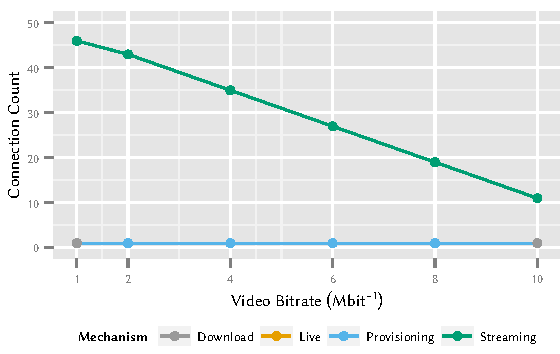
\includegraphics{application/lte_video/numerical_evaluation/figures/bitrate2connections}
  \caption{Influence of bitrate and download mechanism on connection counts.}
  \label{fig:application:lte_video:numerical_evaluation:energy_consumption:bitrate2connections}
\end{figure}

In \reffig{fig:application:lte_video:numerical_evaluation:energy_consumption:bitrate2connections} we study the impact of the different transmission mechanisms on the number of connections per transmission and thus the amount of generated signalling.
We observe that for the transmission mechanisms download, live, provisioning the number of connections is constantly one, independent of the selected bitrate \bitrate.
This is due to the fact that in these transmission mechanisms the video is transmitted in one chunk.
For streaming, the number of connections decreases as the video bitrate increases.
Here, a connection occurs each time the buffer is refilled.
For larger bitrates, refilling the buffer requires a longer transmission.
As the maximum time of video transmission is upper bounded by the video length, longer buffering phases result in a smaller total amount of buffering phases and thus in less connections per video transmission.

\begin{figure}
  \centering
  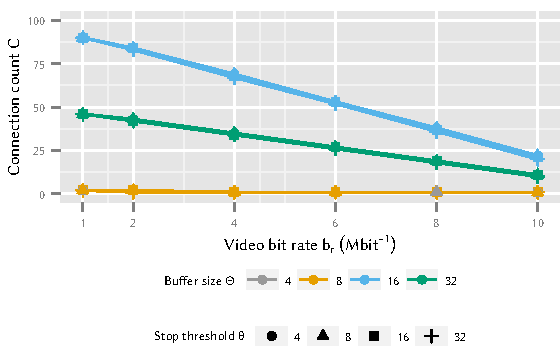
\includegraphics{application/lte_video/numerical_evaluation/figures/bitrate2connections_parameters}
  \caption{Influence of bitrate and selected parameters on connection counts for the streaming mechanism. Lines for different Stop Thresholds \(\theta\) overlap.}
  \label{fig:application:lte_video:numerical_evaluation:energy_consumption:bitrate2connections_parameters}
\end{figure}

Next, we consider the impact of the stop threshold~\bufferlower and buffer size~\buffersize on the number of connections \connectioncount caused by the \streaming mechanism.
In \reffig{fig:application:lte_video:numerical_evaluation:energy_consumption:bitrate2connections_parameters} we observe that while the buffer size has a significant impact on the number of connections during a video transmission, the lower buffer threshold has almost no impact.
For buffer sizes of \SIrange{4}{8}{\second}, no new connections are started, i.e. no signalling occurs.
This is due to the fact that the connection timeout in \gls{UE} is configured as \SI{11.576}{\second}, as discussed in \refsec{sec:application:lte_video:system_model:lte_network_model}.
Thus, for this low buffer sizes the \gls{UE} does not disconnect from the network.
Furthermore, we observe that as the buffer size increases, the number of connections decreases.
Refilling larger buffers requires, similar to larger bitrates, longer transmission times.
Thus, due to the total upper bound on the transmission time, less download phases can occur during the transmission.
\subsection{Trade-Offs}\label{sec:application:lte_video:trade_offs}
\subsubsection*{Transmission Mechanism Selection}\label{sec:application:lte_video:trade_offs:mechanism_selection}
\subsubsection*{Influence of Buffer Threshold Selection}\label{sec:application:lte_video:trade_offs:buffer_threshold_influence}

\begin{figure}
  \centering
  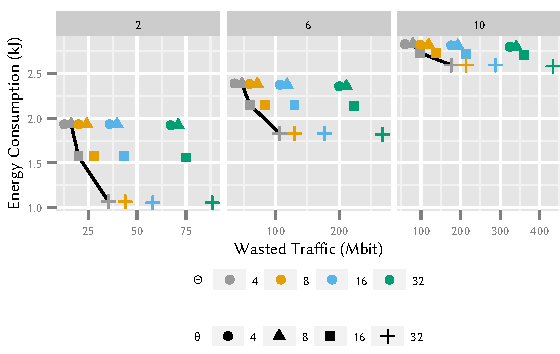
\includegraphics{application/lte_video/trade_offs/figures/energy2lostData}
  \caption{Evaluation of the streaming mechanism for varying video bitrates regarding energy consumption and wasted traffic}
  \label{fig:application:lte_video:numerical_evaluation:trade_offs:energy2lostData}
\end{figure}

\begin{figure}
  \centering
  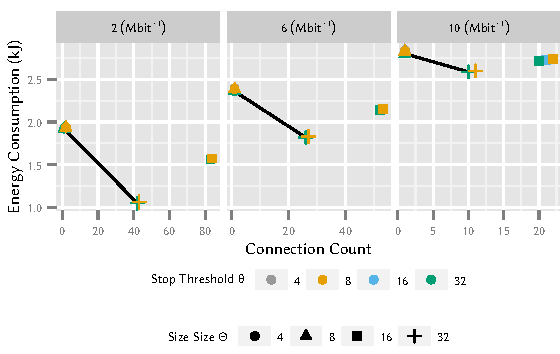
\includegraphics{application/lte_video/trade_offs/figures/energy2connections}
  \caption{Evaluation of the streaming mechanism for varying video bitrates regarding energy consumption and signalling}
  \label{fig:application:lte_video:numerical_evaluation:trade_offs:energy2connections}
\end{figure}

\begin{figure}
  \centering
  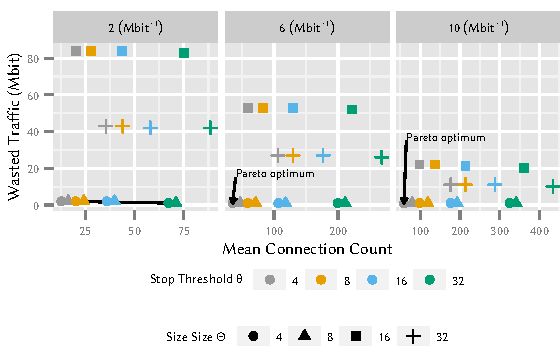
\includegraphics{application/lte_video/trade_offs/figures/connections2lostData}
  \caption{Evaluation of the streaming mechanism for varying video bitrates regarding signalling and wasted traffic}
  \label{fig:application:lte_video:numerical_evaluation:trade_offs:connections2lostData}
\end{figure} 